\subsection{Artifacts}

Finalmente, analizaremos los llamados ``artifacts'', los cuales podr\'ian ser definidos como alteraciones anormales de los videos. Sin embargo, generar estos artifacts puede llegar a ser d\'ificil dado que no solo requiere de varias combinaciones de pruebas y videos, sino tambi\'en agudizar la vista para poder encontrarlos. Ante esto, decidimos tomar como estrategia para poder encontrarlos y analizarlos, quitar 1, 5 y 10 frames de los videos originales y generarlos con los 3 m\'etodos. Esto lo haremos con todos los videos para poder encontrar estos artifacts.

Luego de realizar las pruebas, y analizar los frames y videos generados detectamos lo siguiente para cada m\'etodo:

\begin{enumerate}
\item M\'etodo m\'as cercano: al elevar el n\'umero de frames que generamos con este m\'etodo, el resultado es equivalente a un slide de im\'agenes est\'aticas, esto es, muchos frames iguales por segundo. Este efecto era esperable dado que este m\'etodo genera un nuevo frame id\'entico al frame m\'as cercano, por lo cual ejecutarlo para generar muchos frames entre frames originales (10 en el caso de nuestras pruebas) solo generar\'a copias de \'estos frames originales. Esto es un artifact, ya que consideramos que se pierde la esencia del video, que es el movimiento continuo, y que es remplazado por im\'agenes est\'aticas que se pasan lentamente.
\item M\'etodo interpolaci\'on lineal: en este m\'etodo pudimos detectar un efecto al que vamos a llamar ``ghosting'', y que lo vamos a definir como el frame generado por la superposici\'on del frame anterior y el siguiente del que presenta este efecto. Este efecto sucede debido a que al ocurrir cambios bruscos entre frames, interpolaci\'on lineal intentar\'a generar un frame intermedio entre ambos. Si bien este efecto es d\'ificil de apreciar cuando solo generamos 1 frame entre frames (dado que se necesita ver el video frame a frame para apreciarlo), al aumentar la cantidad de frames a generar en 5 o 10, el efecto se vuelve mucho m\'as notorio. El efecto se puede apreciar en la figura 1.

\begin{figure}[H]
  \centering
    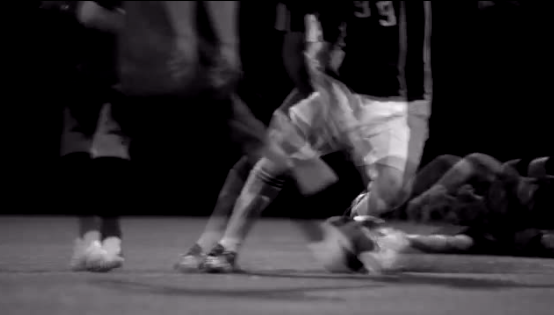
\includegraphics[width=0.5\textwidth]{img/artifact_lineal.png}
  	\caption{Ghosting, el artifact de interpolaci\'on lineal.}
\end{figure}

M\'as a\'un, cuando generamos de a 10 frames entre frames originales, se produce un efecto relativamente similar al que se produce con el m\'etodo del m\'as cercano: el video se convierte en un slide de im\'agenes. Sin embargo, esta vez, el paso de una imagen a la otra de este slide tiene un efecto de transici\'on, el cual el frame actual se va ``desvaneciendo'' mientras que el siguiente se ``aparece'', por lo cual lo consideramos como otro artifact.

\item M\'etodo splines: para el video generado por este momento, detectamos que se genera el mismo efecto de ghosting que en con interpolaci\'on lineal, dado que tambi\'en es un tipo de interpolaci\'on. Sin embargo, hemos detectado una alteraci\'on extra. Esta alteraci\'on produce un efecto interesante, por el cual luego de un efecto de ghosting en los frames de la transici\'on de un cambio de c\'amara, el frame anterior al cambio de c\'amara vuelve a aparecer en negativo en superposici\'on con los frames luego del cambio de c\'amara. Para apreciar este efecto, se pueden observar las figuras 2 y 3.

\begin{figure}[H]
  \centering
    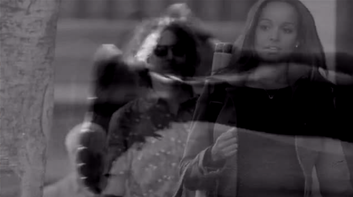
\includegraphics[width=0.5\textwidth]{img/ghosting_splines_1.png}
  	\caption{Ghosting en splines para el cambio de c\'amara.}
\end{figure}

\begin{figure}[H]
  \centering
    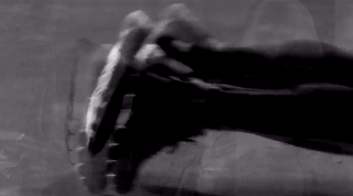
\includegraphics[width=0.5\textwidth]{img/ghosting_negative.png}
  	\caption{Frame en negativo con superposici\'on con otro frame en splines.}
\end{figure}

\end{enumerate}

Adem\'as, realizamos otros experimentos interpolando varios frames entre cada par de frames del video original, pero no logramos obtener alg\'un efecto distinto a los ya mencionados. Incluso experimentamos con videos sin cambios de c\'amara, pero sin nuevos resultados.
